Para la experimentación se utilizó una máquina Desktop Intel(R) Core(TM) i5-4570T CPU @ 2.90GHz, 5.7G Ram, con DB: 5.5.46-MariaDB-1ubuntu0.14.04.2.

El análisis que se realiza de los resultados obtenidos es comparando la calidad de los resultados de los algoritmos discutidos en \autoref{chap:desarrollo}, sobre las bases de datos de \autoref{chap:busquedas}. Con el objetivo de evaluar las propuestas algorítmicas, se consideraron los siguientes métodos:

\begin{itemize}
\item{$alg1$} PAC(C-HAC / selección simple)
\item{$alg2$} PAC(BOBO-10 / selección simple)
\item{$alg3$} PAC(BOBO-10 / selección proporcional)
\item{$alg4$} PAC(BOBO-10 / selección proporcional) + tabú
\item{$alg5$} PAC(Intra-Inter C-HAC / selección proporcional)
\item{$alg6$} PAC(Intra-Inter C-HAC / selección proporcional) + tabú
\item{$alg7$} Construcción golosa
\item{$alg8$} Construcción golosa + tabú
\end{itemize}

Tanto $alg1$ como $alg2$ corresponden a metodologías propuestas en \cite{compositeRetrival}. Los otros algoritmos involucran las mejoras propuestas en este trabajo, para PAC es \texttt{Intra-Inter C-HAC} en la etapa de producción y la selección proporcional en la etapa de selección. En los casos que se agregá la búsqueda tabú, En \texttt{PAC} se realiza la búsqueda tabú \texttt{Inter-Paquete} luego de la etapa de producción y la \texttt{Intra-Paquete} luego de la selección. En la \texttt{Búsqueda Golosa} de la solución obtenida se realiza la búsqueda tabú \texttt{Intra-Paquete}. Cabe señalar que no se tienen en consideración BOBO-Ex y CAP ya que para el tamaño de la instancia los tiempos de ejecución de esos algoritmos resultaron prohibitivos. A partir de experimentación preliminar con BOBO para valores $c=1, 5$ y $10$, resultó $c=10$ la opción más competitiva. Para la búsquedas tabú se definió que la cantidad de iteraciones de permanencia de un elemento en la lista tabú sea el promedio de elementos que tiene un paquete en la solución inicial.

Para realizar una comparación entre la calidad de las soluciones obtenidas por los diferentes algoritmos, se ha evaluado para los $\gamma \in \left\{0,1; 0,3; 0,4; 0,5; 0,6; 0,7; 0,8; 0,9\right\} $el porcentaje de deterioro de cada solución.

En el caso de la búsqueda de artículos, que es el escenario que contiene la mayor cantidad de objetos, los tiempos de ejecución  para los algoritmos C-HAC ($alg1$, $algo5$ y $alg6$) son del orden de los 5 minutos, mientras que para los algoritmos BOBO ($alg2$, $alg3$ y $alg4$) de 2 minutos y los golosos ($alg7$ y $alg8$) de los x minutos. Los incrementos de tiempo debido a la ejecución de las metaheruísticas de mejora son despreciables, están entre los 5 y 7 segundos. Por lo cual no se considera que el tiempo sea un factor que valga la pena analizar.

\section{Base de datos de artículos}
Para comprender el comportamiento de los resultados de las búsquedas se diseñaron dos tipos de gráficos que permiten visualizar la cohesión de los paquetes y la distancia entre ellos. De esta forma se podrá analizar la calidad del resultado obtenido más allá del valor de la función objetivo.

Los gráficos del estilo de la figura \ref{res:img-explain-bars} permiten analizar la distribución de los tópicos de una solución a nivel de paquete y de la relación con otros. Las filas corresponden a los 10 paquetes obtenidos y las columnas a los 38 tópicos considerados. El tamaño del círculo representa la proporción del tópico en el perfil del artículo y el color hace referencia al paquete al cual artículo pertenece. Por lo tanto, dos artículos tendrán gran similitud cuando los patrones de sus círculos coincidan, tanto en tamaño como en distribución. Si para un paquete la distribución entre los tópicos y el tamaño de los círculos es similar entre sus artículos se puede deducir que este paquete es cohesivo (tiene buen valor intra). Por otro lado, si los patrones de los círculos de los dos artículos más similares entre distintos paquetes no coinciden, esto indica que el resultado es diverso.
\begin{figure}[H]
  \centering
    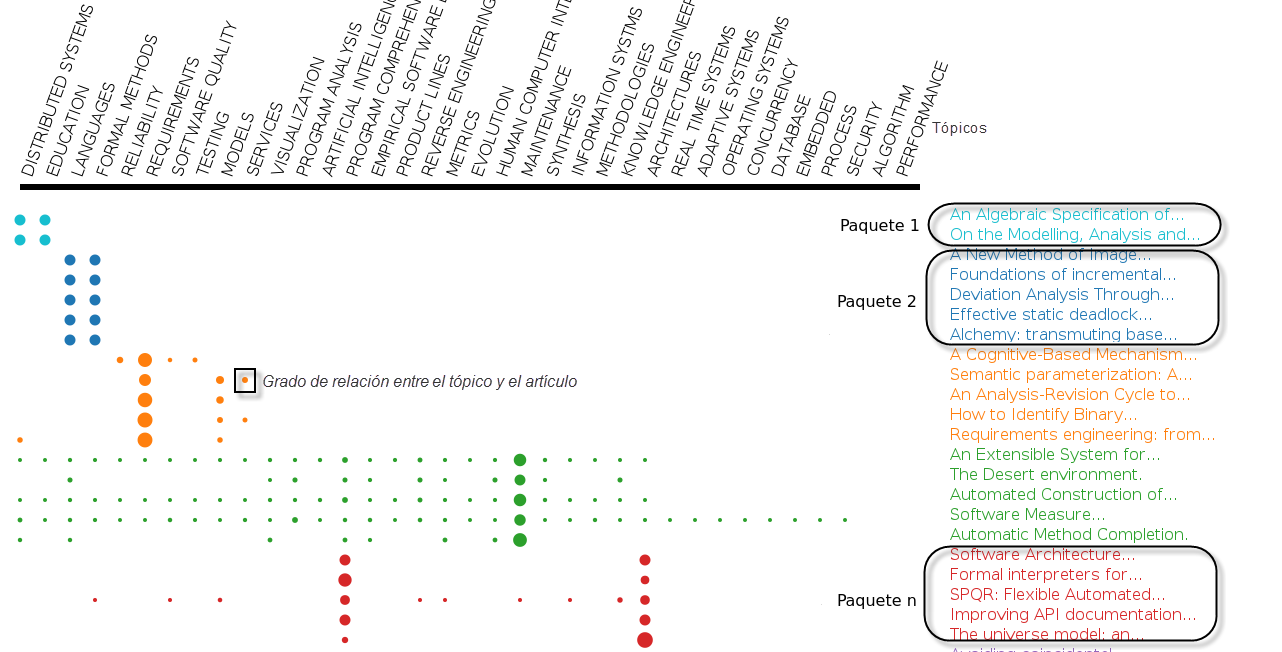
\includegraphics[width=1\textwidth]{img/explain-bars.png}
  \caption{}
  \label{res:img-explain-bars}
\end{figure}

Los gráficos de tipo burbuja de la figura \ref{res:img-explain-bubbles} son útiles para concluir el nivel de acoplamiento entre los paquetes de una solución, observando la relación entre los tópicos y los paquetes. Cada burbuja representa un tópico que contiene círculos; cada circulo es un artículo donde el tamaño es la proporción del articulo con el tópico y el color el paquete al que pertenece. Entonces si las burbujas contienen círculos de más de un color se puede decir que ese resultado no es muy diverso, mientras que el color de los círculos de las burbujas sea más homogéneo el resultado es más diverso. En cuanto a la cohesión de los paquetes, es más cohesivo cuando el tamaño de cada circulo dentro de cada burbuja sea similar (para el mismo color) y la distribución de los círculos entre cada burbuja es equitativa.

\begin{figure}[H]
  \centering
    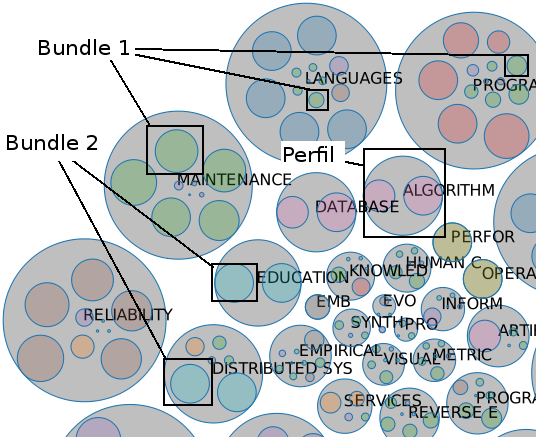
\includegraphics[width=0.5\textwidth]{img/explain-bubbles.png}
  \caption{}
  \label{res:img-explain-bubbles}
\end{figure}


\subsection{Búsqueda de artículos}
Para la búsqueda de artículos con tópicos similares en la tabla \ref{tabla:comp1} se observa los porcentajes de deterioro de cada solución respecto de la mejor solución obtenida por alguno de los ocho algoritmos. Una primera observación es que los algoritmos  Intra-Inter C-HAC reflejan el efecto buscado: a menores valores de $\gamma$ donde el valor inter tiene mayor peso, se obtienen mejores soluciones. Es decir, haber considerado en el proceso de generación de paquetes la funcion Intra-Inter benefició a la calidad de las soluciones obtenidas. Claramente, a medida que $\gamma$ crece y la función intra adquiere mayor preponderancia, la función $Score$ tiene mejor performance. Los algoritmos BOBO, no obtienen soluciones de la calidad de los algoritmos C-HAC y el proceso de selección proporcional no logra una mejora consistente para todos los valores de $\gamma$. Las soluciones obtenidas con el algoritmo de construcción golosa, no alcanzaron a mejorar las soluciones de C-HAC pero fueron ampliamente mejores que las de BOBO. En promedio el porcentaje de deterioro de BOBO fue de un $50\%$ mientras que el goloso fue de un $12\%$. 
Cabe resaltar el muy buen rendimiento de la búsqueda tabú, tanto en escenarios donde la solución inicial no es de buena calidad (algoritmo BOBO) así como también considerando soluciones de mejor calidad (algoritmo Intra-Inter C-HAC). En el primer caso, se obtienen porcentajes de mejora por encima del $70\%$. En el segundo caso, para varios valores de $\gamma$ la solución obtenida por la búsqueda tabú resultó ser la mejor opción y en otros con deterioros inferiores al $0.5\%$.
\begin{table}
\begin{center}
\begin{tabular}{|c|c|c|c|c|c|c|c|c|}
\hline
$\gamma$&$alg1$&$alg2$&$alg3$&$alg4$&$alg5$&$alg6$&$alg7$&$alg8$ \\ \hline
0.1 & -2.34	& -35.06 & -37.11 & -13.48 & -0.72 &  0.00 &  -4.82 &  -4.38 \\
0.2 & -2.45	& -40.01 & -40.05 & -6.28 & -0.35 &  0.00 &  -5.25 &  -4.46 \\
0.3 & -3.39	& -44.54 & -44.50 & -11.63 & -1.10 &  0.00 & -10.16 &  -9.09 \\
0.4 & -0.45	& -48.85 & -50.16 & -3.00 & -0.31 &  0.00 & -10.68 &  -9.95 \\
0.5 & 0.00  & -52.32 & -52.62 & -7.38 & -0.31 & -0.02 & -12.97 & -12.07 \\
0.6 & -0.19 & -55.57 & -54.98 & -6.83 & -0.24 &  0.00 & -14.94 & -13.97 \\
0.7 & 0.00  & -57.11 & -56.52 & -9.36 & -0.41 & -0.21 & -16.21 & -15.19 \\
0.8 & 0.00  & -57.90 & -57.83 & -6.08 & -0.56 & -0.41 & -18.10 & -16.99 \\
0.9 & 0.00  & -58.51 & -58.44 & -6.41 & -0.48 & -0.23 & -20.47 & -19.31 \\ \hline 
\end{tabular}
\caption{Comparación de calidad de soluciones entre algoritmos} 
\label{tabla:comp1}
\end{center}
\end{table}

Como se señaló previamente, la búsqueda tabú tiene su mayor impacto cuando es aplicada a la solución brindada por el algoritmo $alg5$ y en este contexto resulta una buena alternativa por su bajo costo computacional. 

Para $\gamma=0.1$, la Figura~\ref{res:bobo} muestra que la solución dada por el $alg5$ tiene artículos de distintos paquetes con patrones muy similares, indicando un bajo valor inter-paquete. Por el contrario, luego de aplicar la búsqueda tabú los patrones de los artículos más similares entre distintos paquetes se volvieron más dispares, demostrando el aumento de la diversidad entre paquetes. Para $\gamma=0.9$, como puede observarse en la misma Figura~\ref{res:bobo}, en la solución brindada por el $alg5$ todos los paquetes tienen al menos un artículo cuyo patrón consiste en muchos pequeños círculos distribuídos en la mayoría de los tópicos en contraposición al resto de los artículos del mismo paquete con pocos círculos de gran tamaño. Esto muestra bajo valor intra-paquete. Mientras que los paquetes obtenidos luego de aplicar la búsqueda tabú son mucho más cohesivos ya que los círculos de los artículos dentro de un mismo paquete siguen patrones mucho más parecidos. Esto demuestra que la búsqueda tabú fue capaz de mejorar las características de la solución en función del parámetro $\gamma$.

Como se mencionó anteriormente, el algoritmo $C-HAC$ de \cite{compositeRetrival} ($alg1$) utiliza la función $Score$ para la decisión del par de {\em clusters} a unir en la etapa de producción de paquetes y la selección simple en la segunda fase. Estos dos criterios omiten la diversidad de los paquetes. De acuerdo a los resultados de la tabla \ref{tabla:comp}, se pudo concluir que haber considerado la función Intra-Inter y la selección proporcional benefició a la calidad de las soluciones cuando la misma es medida a partir de la función objetivo $w(S)$. Con el fin de evaluar que el $alg4$ es capaz de captar efectivamente la diversidad en la solución, se analiza las soluciones para $\gamma=0.5$. En este caso el $alg1$ obtuvo un valor de $intra=93.82$ y de $inter=35.49$, mientras que el $alg4$ logró valores de $intra=93.86$ y de $inter=37.69$. Estos valores demuestran que el $alg4$ es capaz de encontrar soluciones con mayor valor $inter$ sin causar un deterioro en el valor $intra$. Observando la Figura~\ref{res:chac} se puede ver que la cohesión intra-paquete de ambas soluciones es equivalente. Sin embargo, la diversidad en la segunda solución es mayor, ya que los patrones entre los artículos más similares de distintos paquetes son más heterogéneos. 

\subsection{Búsqueda de autores}
\section{Búsqueda de atracciones turísticas}\label{res:busAtracciones}
Los resultados son conjuntos de paquetes que cada uno contiene atracciones turísticas de distinta temática, que son similares con respecto a la distancia geográfica y la suma del precio de las atracciones no supera el presupuesto.
\begin{itemize}
  \item \textbf{Similitud}: Cercanía geográfica de las atracciones.
  \item \textbf{Complementariedad}: Tipo de atracción turística.
  \item \textbf{presupuesto}: Cantidad de dinero que tiene el usuario para utilizar.
\end{itemize}
Se generaron soluciones con las siguientes características:\\

\SolucionBudget
{}
{
\begin{description}
	\item[alg\_1] \texttt{Búsqueda Golosa}
	\item[alg\_2] \texttt{PAC(BOBO-100/Selección de paquetes proporcional)}
	\item[alg\_3] \texttt{PAC(BOBO-100/Selección de paquetes)}
	\item[alg\_4] \texttt{PAC(Efficient C-HAC/Selección de paquetes proporcional)}
	\item[alg\_5] \texttt{PAC(Efficient C-HAC/Selección de paquetes)}
\end{description}
}
{$(0,1; 0,3; 0,5; 0,7; 0,9)$}
{10}
{3}
{7}

\begin{figure}[H]
  \centering
    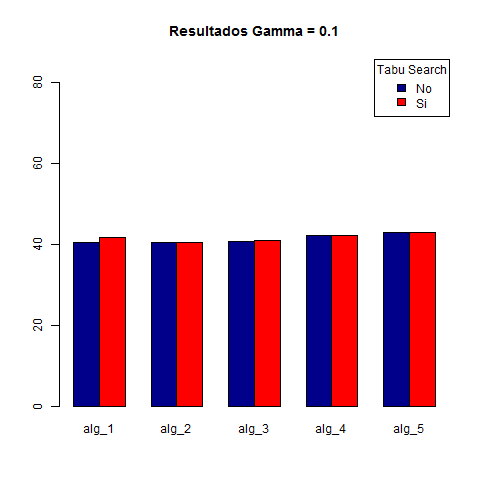
\includegraphics[width=0.8\textwidth]{resultados/cities/Graficos_agrupados/gamma01-cities.png}
  \caption{Función Objetivo $\gamma$ = $0.1$ vs Algoritmos de resolución}
  \label{res:img-cities-agr-gamma01}
\end{figure}

\begin{figure}[H]
  \centering
    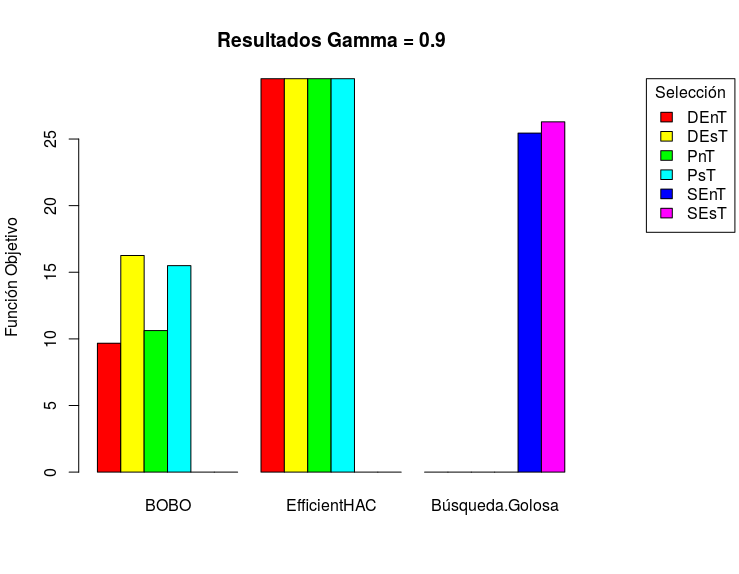
\includegraphics[width=0.8\textwidth]{resultados/cities/Graficos_agrupados/gamma09-cities.png}
  \caption{Función Objetivo $\gamma$ = $0.9$ vs Algoritmos de resolución}
  \label{res:img-cities-agr-gamma09}
\end{figure}

En esta instancia se repite el comportamiento de los resultados obtenidos en las consultas realizadas sobre la base de datos de artículos. La solución del algoritmo goloso supera al de PAC cuando la estrategia de producción es con BOBO pero con HAC valor de la función objetivo es similar. También, en esta instancia, se obtuvieron mejores valores con la selección proporcional.

Al aplicar la búsqueda tabú se mejora sustancialmente la solución obtenida con PAC con la estrategia BOBO, obteniendo una solución tan optima como con el resto de los algoritmos. Con el resto de los algoritmos no se obtiene una mejora sustancial de la solución al aplicar la búsqueda tabú.

Solo se muestran los gráficos y comportamientos para las pruebas realizadas con un solo presupuesto, pero los mismos tuvieron el mismo efecto a medida que se cambiaba ese valor.
